\section{Resultados}

\subsection{Experimentos Planteados}



\begin{wrapfigure}{r}{0.5\textwidth}
  \vspace{-20pt}
  \begin{center}
    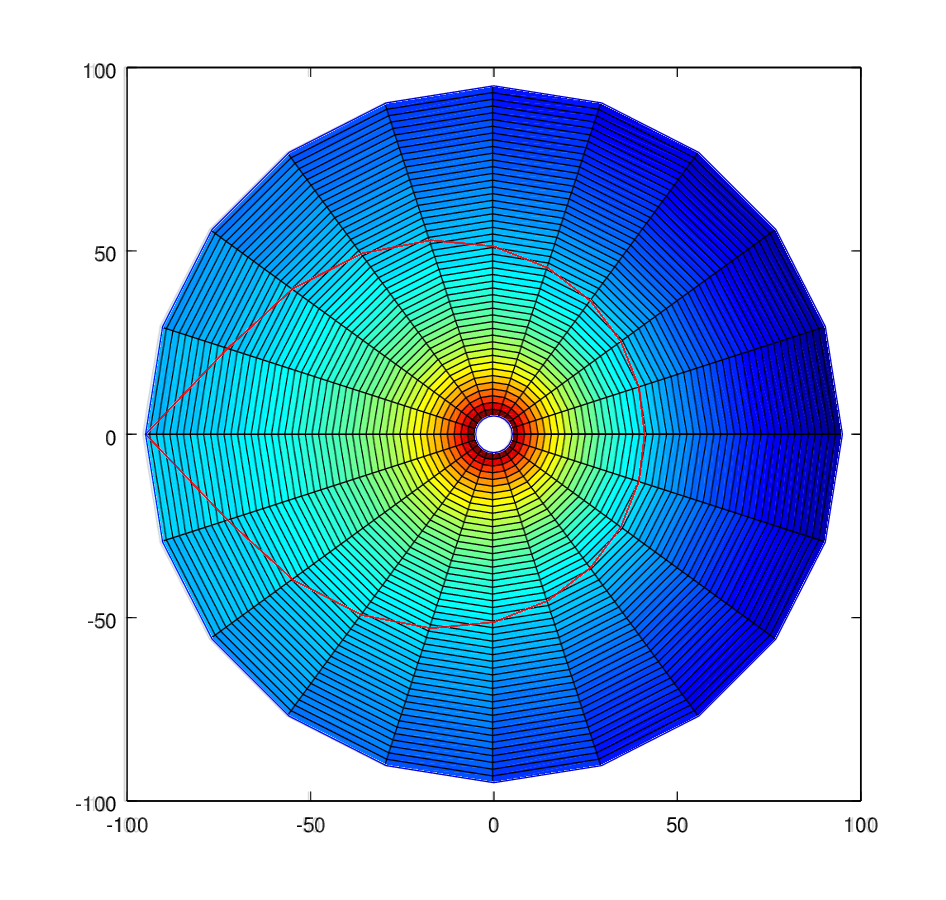
\includegraphics[scale= 0.4]{imagenes/hornoColorSubeBajaConIsoterma.png}
  \end{center}
  \vspace{-20pt}
  \caption{Experimento 1}
  \vspace{-10pt}
  \label{fig:Exp1}
\end{wrapfigure}

El primer experimento planteado consistió en generar una instancia del problema donde los valores de las tmperaturas externas varien gradualmente desde 0 hasta la isoterma pedida. Para esto generamos una instancia con $n=20$, donde para el primer ángulo, la temperatura de la pared externa vale $0$ y luego aumenta en sentido anti-horario en 50. Al llegar a la mitad de la circunferencia, llega a valer 500 y luego decrece nuevamente. La idea de este experimento consistió en ver la variación de la isoterma y además aprovechar esta variación para estudiar para cada ángulo, la variación de la temperatura para cada punto obtenido.
\\
\begin{wrapfigure}{r}{0.5\textwidth}
  \vspace{-20pt}
  \begin{center}
    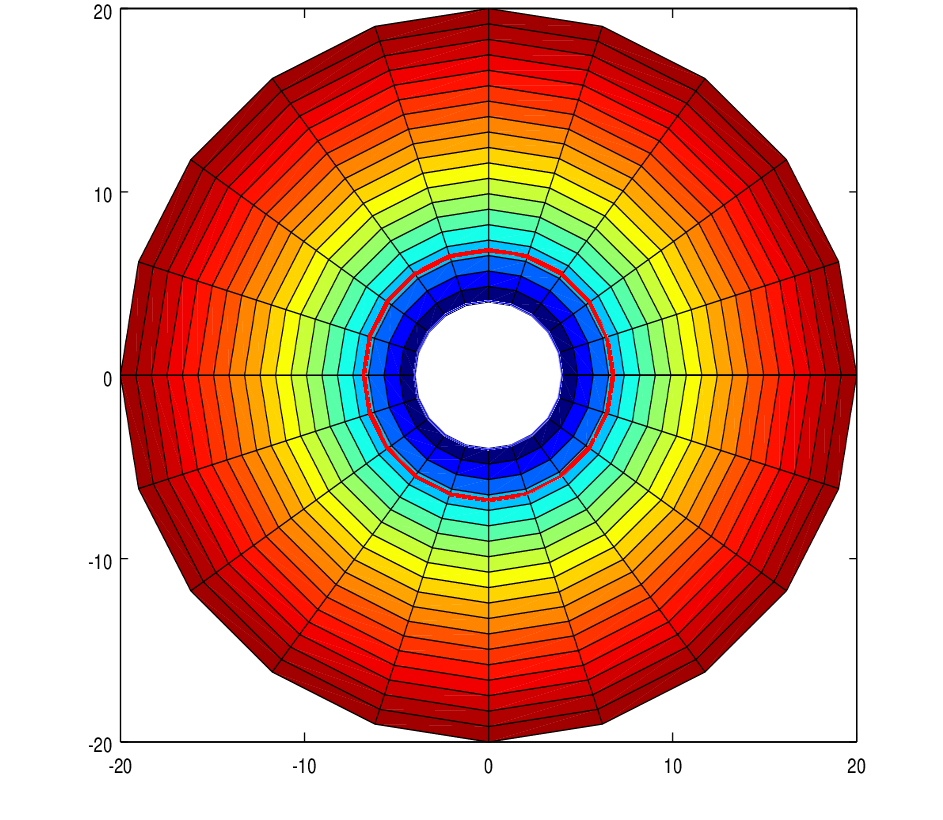
\includegraphics[scale= 0.4]{imagenes/hornoInvertidColoroConIso.png}
  \end{center}
  \vspace{-20pt}
  \caption{Experimento 2}
  \vspace{-10pt}
  \label{fig:Exp1}
\end{wrapfigure}

El segundo experimento planteado consistió en generar una instancia del problema donde los valores de las temperaturas se encuentren invertidas, es decir, las temperaturas internas son menores que las externas. Para esto generamos una instancia con $n=20$, con las paredes internas valiendo 0 y las externas valiendo 1500. La idea de este experimento consistió en ver si el la ecuación planteada seguía teniendo sentido y si nos topabamos con una solución razonable del sistema o si nos encontraríamos con algun error.
\\
%Para ambas figuras se marcaron los valores de la isoterma encontrada
\begin{wrapfigure}{l}{0.5\textwidth}
  \vspace{-20pt}
  \begin{center}
    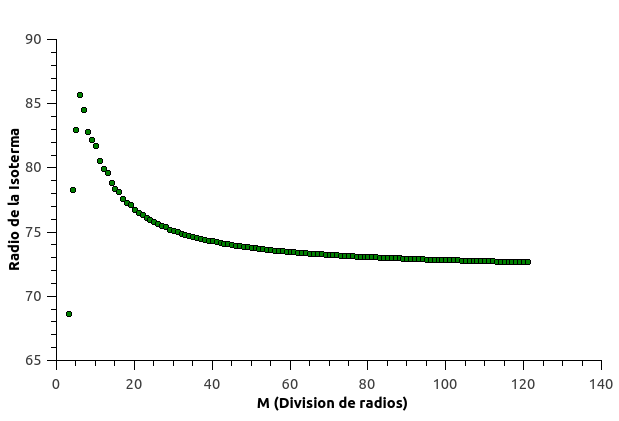
\includegraphics[scale= 0.4]{imagenes/graphDiscretizacionv2.png}
  \end{center}
  \vspace{-20pt}
  \caption{Experimento 3}
  \vspace{-10pt}
  \label{fig:Exp3}
\end{wrapfigure}

El tercer experimento planteado consistió en estudiar el impacto de incrementar la discretización de los radios (aumentar el $m$) y ver como impacta en la obtención de la isoterma. Se uso una instancia donde los valores internos valen 1500, los externos valen 0 y la diferencia entre el radio interno y el externo es 100. Empezamos tomando $m=3$ y lo aumentamos de a 1 hasta llegar a $m=120$, manteniendo todos los parametros igual. De este modo, podemos observar como impacta la discretización del radio en el valor del radio obtenido de la isoterma.\\
%Una instancia del problema equivale a un corte del horno como se ilustra en la figura ~\ref{fig:Exp1}. Dado que la medición de temperatura en el horno puede realizarse en infinitos puntos, discretizamos el problema fijando la ubicación de los mismos de la siguiente manera; Dividimos el horno en \textbf{\textit{n}} cantidad de ángulos de tamaño $\Delta_{\theta}$ y en \textbf{\textit{m + 1}} cantidad de radios, de tamaño $\Delta_{r}$. Analizaremos las temperaturas en los puntos donde se unen las divisiones entre ángulos y radios. Recordemos que los puntos de la pared interna y externa son dato.\\
%\\